\Variant{28.04.2024}
\QQ{1}{$x$, $y$, $z$ natural sonlar uçun $\dfrac{2x+3y}6=z$ bölsa, $x$ quyidagi sonlardan qaysi biriga qoldiqsiz bölinadi?
\Opts{$2$}{$3$}{$4$}{$6$}}
\QQ{2}{Hisoblang:
\[\left(1-\left(1-\left(1-\left(1-2^{-2}\right)^{-1}\right)^{-3}\right)^{-1}\right)^{-1}\]
\Opts{$27$}{$28$}{$\dfrac{28}{27}$}{$\dfrac{27}{28}$}}
\QQ{3}{Oltin va kumuş qotişmasining massasi $1{,}06$ kg. Qotişmani suvga solinganda $70$ gr massasini yöqotadi. Oltin suvda massasining $\dfrac1{19}$ qismini, kumuş esa $\dfrac1{10}$ qismini yöqotadi. Oltin va kumuşning dastlabki massalarini toping.
\Opts{Oltin $760$ gr, kumuş $300$ gr}{Oltin $560$ gr, kumuş $500$ gr}{Oltin $300$ gr, kumuş $760$ gr}{Oltin $500$ gr, kumuş $560$ gr}}
\QQ{4}{Avtomobilning narxi $10\,000$\,\$ edi. Narx ketma-ket $15\%$ ikki marta oşirilgandan keyin avtomobilning narxi qança böladi?
\Opts{$12\,000$}{$11\,500$}{$12\,225$}{$13\,225$}}
\QQ{5}{$3^8\cdot3^{-2}\cdot2^{-4}\cdot2^8=2^m\cdot3^n$ bölsa, $m+n$ ni toping.
\Opts{$6$}{$8$}{$10$}{$12$}}
\QQ{6}{Hisoblang:
\[\sqrt{22-30\sqrt{4-2\sqrt3}}+5+3\sqrt3\]
\Opts{$10$}{$6\sqrt3$}{$12$}{$5-3\sqrt3$}}
\QQ{7}{Hisoblang:
\[\frac3{2\sqrt[3]2+2\sqrt[3]4}-\frac3{2\sqrt[3]2-2\sqrt[3]4}+\sqrt[3]4\]
\Opts{$\sqrt[3]4$}{$\sqrt[3]{16}+1$}{$\left(\sqrt[3]4+1\right)^2$}{$-\left(\sqrt[3]4+1\right)^2$}}
\QQ{8}{Agar $a=1{,}9$, $b=0{,}55$ bölsa, quyidagi ifodaning qiymatini toping.
\[\frac{a^2-4b^2-5a+10b}{(a+2b)^2-25}\]
\Opts{$10$}{$0{,}1$}{$0{,}01$}{$1$}}
\QQ{9}{Kamayuvçi arifmetik progressiyada $a_3=1$ va $a_5^2=25$ bölsa, $a_1\cdot d$ ning qiymatini toping.
\Opts{$-14$}{$-21$}{$-6$}{$4$}}
\QQ{10}{$b_n=\dfrac{2^n}{3^{n-1}}$ berilgan ketma-ketlikning hadlari yiğindisini toping.
\Opts{$2$}{$4$}{$6$}{$8$}}
\QQ{11}{$\sqrt{x-2}+\sqrt{1-x}=2$ tenglama neçta haqiqiy ildizga ega?
\Opts{$1$}{$2$}{Çeksiz köp}{Yeçimga ega emas}}
\QQ{12}{$\left(\sqrt5+2\right)^{x-1}\le\left(\sqrt5-2\right)^{\frac{x-1}{x+1}}$ tengsizlikning musbat butun yeçimlari neçta?
\Opts{$1$}{$2$}{$3$}{$4$}}
\QQ{13}{$2^{\ln x}-3^{\frac12\ln x}=1$ tenglama neçta ildizga ega?
\Opts{Çeksiz köp}{$1$}{$2$}{Yeçimga ega emas}}
\QQ{14}{$\left|x^2-x-6\right|>0$ — neçta natural son tengsizlikning yeçimi böla olmaydi?
\Opts{$0$}{$1$}{$2$}{$3$}}
\QQ{15}{$2^a=3$, $2^b=5$ va $\left(\dfrac{25}3\right)^c=405$ bölsa, $c$ ni $a$ va $b$ orqali ifodalang.
\Opts{$\dfrac{2a-b}{2b-a}$}{$\dfrac{4a-b}{4a+b}$}{$\dfrac{2b-a}{4a-b}$}{$\dfrac{4a+b}{2b-a}$}}
\QQ{16}{Ifodani soddalaştiring:
\[\frac{(\sin x-\cos x)^2}{\sin^2\left(\frac\pi4-x\right)}\]
\Opts{$2$}{$\dfrac{1-\sin2x}{1+\sin2x}$}{$\dfrac{2(1-\sin2x)}{1-\cos2x}$}{$1$}}
\QQ{17}{$\sqrt3\sin2x-\cos2x=\sqrt3$ tenglama $(0;\,5\pi)$ oraliğida neçta ildizga ega?
\Opts{$20$}{$18$}{$10$}{$8$}}
\QQ{18}{$\dfrac{-2}{|x|+1}\ge|x|-2$ tengsizlikning butun yeçimlari neçta?
\Opts{$0$}{$1$}{$2$}{$3$}}
\QQ{19}{$g(x)=3x^3-x^2-x+4$ bölsa, $g\left(\dfrac{1+\sqrt{13}}6\right)$ ning qiymatini toping.
\Opts{$0$}{$3$}{$4$}{$5$}}
\QQ{20}{Çizmada $f(x)$ va $g(x)$ funksiya grafiklari tasvirlangan. $x_1$, $x_2$, $x_3$, $x_4$, $x_5$, $x_6$ nuqtalarning neçtasida $f'(x)\cdot g(x)\ge0$ tengsizlik örinli böladi?
\qfig{\begin{tikzpicture}[x=0.6cm,y=0.7cm,font=\small]
\draw[-{Stealth[length=4pt]}] (-5.8,0)--(5.9,0) node[right] {$x$}; \draw[-{Stealth[length=4pt]}] (0,-1.9)--(0,2) node[left] {$y$};
\draw[thick,domain=-5.4:5.3,samples=120] plot (\x,{1.4*cos(deg(2*pi*(\x+0.05)/4))}); \node at (-2.4,-1.6) {$f(x)$};
\draw[thick] (-5.6,1.4)--(5.6,-1.4); \node[above] at (-5.2,1.35) {$g(x)$};
\foreach \t/\n in {-4.6/1,-3.5/2,-0.5/3,0.5/4,3.4/5,4.5/6} {\draw[dashed] (\t,0)--(\t,{1.4*cos(deg(2*pi*(\t+0.05)/4))}); \node[below] at (\t,0) {\scriptsize$x_\n$};}
\end{tikzpicture}}
\Opts{$5$}{$3$}{$4$}{$6$}}
\QQ{21}{$\displaystyle\int_{\frac\pi3}^{\frac{2\pi}3}x\cdot\sin x\,dx$ aniq integralni hisoblang.
\Opts{$0$}{$\dfrac\pi2$}{$\dfrac\pi4$}{$\pi$}}
\QQ{22}{$\sqrt{3x-2}+15\sqrt[4]{3x-2}=16$ tenglamaning haqiqiy ildizlari köpaytmasini toping.
\Opts{$1$}{$2$}{$4$}{$16$}}
\QQ{23}{$f(x)=ax^2+bx+c$ kvadrat funksiyaning ildizlari $x_1$ va $x_2$ ($x_1<x_2$). Agar $|a|\cdot f(1)<0$, $f(1)\cdot f(2)<0$ va $a\cdot f(2)>0$ bölsa, quyidagi munosabatlardan qaysilari örinli?
\Opts{$x_1<1<x_2<2$}{$1<x_1<2<x_2$}{$1<x_1<x_2<2$}{$x_1<x_2<1<2$}}
\QQ{24}{Aylananing uzunligi $12$ bölsa, şu aylananing uzunligi $3$ ga teng bölgan yoyining gradus ölçovini toping.
\Opts{$90^\circ$}{$60^\circ$}{$45^\circ$}{$30^\circ$}}
\QQ{25}{$ABCDEFGH$ muntazam sakkizburçak. $GHCD$ törtburçak yuzi $12$ bölsa, sakkizburçak yuzini toping.
\qfig{\begin{tikzpicture}[scale=0.85,font=\small]
\coordinate (A) at (-0.5,-1.207); \coordinate (B) at (0.5,-1.207); \coordinate (C) at (1.207,-0.5); \coordinate (D) at (1.207,0.5); \coordinate (E) at (0.5,1.207); \coordinate (F) at (-0.5,1.207); \coordinate (G) at (-1.207,0.5); \coordinate (H) at (-1.207,-0.5);
\fill[qfill] (G)--(H)--(C)--(D)--cycle;
\draw (A)--(B)--(C)--(D)--(E)--(F)--(G)--(H)--cycle; \draw (H)--(C); \draw (G)--(D);
\node[below] at (A) {$A$}; \node[below] at (B) {$B$}; \node[right] at (C) {$C$}; \node[right] at (D) {$D$}; \node[above] at (E) {$E$}; \node[above] at (F) {$F$}; \node[left] at (G) {$G$}; \node[left] at (H) {$H$};
\end{tikzpicture}}
\Opts{$18$}{$24$}{$28$}{$36$}}
\QQ{26}{$x$ ning qabul qilişi mumkin bölgan eng katta natural qiymatini toping.
\qfig{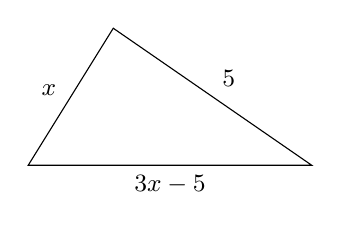
\begin{tikzpicture}[scale=0.6,font=\small]
\draw (0,0)--(6,0)--(1.8,2.9)--cycle;
\node[left] at (0.8,1.6) {$x$}; \node[above right] at (3.9,1.45) {$5$}; \node[below] at (3,0) {$3x-5$};
\end{tikzpicture}}
\Opts{$5$}{$4$}{$3$}{$2$}}
\QQ{27}{$CF=6$, $CG=7$, $GE=5$ va $ED=6$ bölsa, $FG$ kesma uzunligini toping.
\qfig{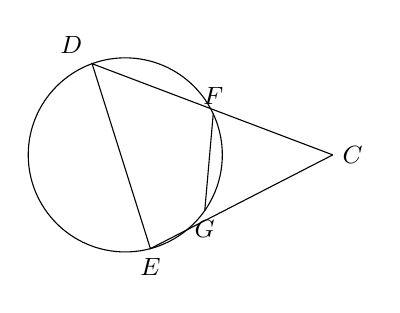
\begin{tikzpicture}[scale=0.85,font=\small]
\coordinate (O) at (0,0); \coordinate (D) at (110:1.45); \coordinate (E) at (-75:1.45); \coordinate (F) at (25:1.45); \coordinate (G) at (-35:1.45); \coordinate (C) at (3.1,0);
\draw (O) circle (1.45); \draw (C)--(D)--(E)--(C); \draw (F)--(G);
\node[above left] at (D) {$D$}; \node[below] at (E) {$E$}; \node[above] at (F) {$F$}; \node[below] at (G) {$G$}; \node[right] at (C) {$C$};
\end{tikzpicture}}
\Opts{$2$}{$3$}{$4$}{$5$}}
\QQ{28}{$ABC$ töğri burçakli uçburçakning katetlaridan kvadratlar hosil qilingan. $M$ nuqta $AC$ ning örta nuqtasi, $N$ nuqta $MB$ töğri çiziq bilan kvadratlarning uçlarini tutaştiruvçi kesmaning kesişiş nuqtasi bölsa, $MN$ kesma uzunligini toping.
\qfig{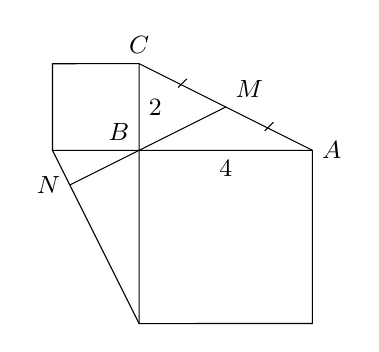
\begin{tikzpicture}[scale=0.55,font=\small]
\coordinate (B) at (0,0); \coordinate (C) at (0,2); \coordinate (A) at (4,0); \coordinate (P) at (-2,0); \coordinate (Q) at (0,-4); \coordinate (M) at (2,1); \coordinate (N) at (-1.6,-0.8);
\draw (B)--(C)--(-2,2)--(P)--cycle; \draw (B)--(A)--(4,-4)--(Q)--cycle; \draw (A)--(C); \draw (P)--(Q); \draw (M)--(N);
\draw (0.9,1.45)--(1.1,1.65); \draw (2.9,0.45)--(3.1,0.65);
\node[above] at (C) {$C$}; \node[above left] at (B) {$B$}; \node[right] at (A) {$A$}; \node[above right] at (M) {$M$}; \node[left] at (N) {$N$};
\node[right] at (0,1) {$2$}; \node[below] at (2,0) {$4$};
\end{tikzpicture}}
\Opts{$\dfrac2{\sqrt5}$}{$\dfrac3{\sqrt5}$}{$\dfrac9{\sqrt5}$}{$\dfrac7{\sqrt5}$}}
\QQ{29}{Çizmada tomoni $4$ ga teng bölgan muntazam oltiburçak tasvirlangan. $\overrightarrow{AB}+\left(\overrightarrow{FE}+\overrightarrow{ED}\right)$ vektorning uzunligini toping.
\qfig{\begin{tikzpicture}[scale=0.45,font=\small]
\coordinate (A) at (-2,-3.464); \coordinate (B) at (2,-3.464); \coordinate (C) at (4,0); \coordinate (D) at (2,3.464); \coordinate (E) at (-2,3.464); \coordinate (F) at (-4,0);
\draw (A)--(B)--(C)--(D)--(E)--(F)--cycle;
\draw[-{Stealth[length=4pt]}] (A)--(B); \draw[-{Stealth[length=4pt]}] (F)--(E); \draw[-{Stealth[length=4pt]}] (E)--(D);
\node[below] at (A) {$A$}; \node[below] at (B) {$B$}; \node[right] at (C) {$C$}; \node[above] at (D) {$D$}; \node[above] at (E) {$E$}; \node[left] at (F) {$F$};
\end{tikzpicture}}
\Opts{$8$}{$8\sqrt7$}{$4$}{$4\sqrt7$}}
\QQ{30}{$ABC$ töğri burçakli uçburçakning $C$ töğri burçak uçidan $AB$ gipotenuzaga parallel tekislik ötkazilgan. Tekislikdan gipotenuzagaça bölgan eng qisqa masofa $12$ ga teng. Katetlarning tekislikdagi proyeksiyalari $16$ va $9$ ga teng bölsa, $AB$ gipotenuza uzunligini toping.
\Opts{$25$}{$30$}{$24$}{$32$}}
\QQ{31}{$A=\{a,\ b,\ c,\ d,\ m,\ n\}$ va $B=\{a,\ b,\ c,\ k,\ l,\ m\}$ töplamlar berilgan. $A\cap B$ töplamning böş bölmagan qism töplamlari soni neçta?
\Opts{$10$}{$8$}{$15$}{$16$}}
\QQ{32}{Tomonlari $8$, $10$, $12$, $14$ sonlaridan (takrorlanişi mumkin) iborat bölgan barça uçburçaklardan tavakkaliga tanlangan uçburçakning muntazam böliş ehtimolini toping.
\Opts{$\dfrac15$}{$\dfrac3{16}$}{$\dfrac25$}{$\dfrac35$}}
\QQ{33}{\Moslash{Ustada bir neçta balandligi asosining diametridan ikki marta katta bölgan bir xil silindr şaklidagi gölalar bor. ($\pi\approx3$ deb oling.)
\par\centering\begin{tikzpicture}[scale=0.5,font=\small]
\draw (0,4) ellipse (1 and 0.25); \draw (-1,0)--(-1,4); \draw (1,0)--(1,4); \draw (-1,0) arc (180:360:1 and 0.25); \draw[dashed] (1,0) arc (0:180:1 and 0.25);
\draw[{Stealth[length=3pt]}-{Stealth[length=3pt]}] (1.4,0)--(1.4,4); \node[right] at (1.4,2) {$2d$}; \draw[{Stealth[length=3pt]}-{Stealth[length=3pt]}] (-1,-0.6)--(1,-0.6); \node[below] at (0,-0.6) {$d$};
\end{tikzpicture}}{A) $\dfrac12$\par B) $1$\par C) $\dfrac13$\par D) $\dfrac23$\par E) $\dfrac14$\par F) $\dfrac34$}{Usta bu göladan iloji boriça eng katta hajmli şar öyib olmoqçi. Bunda şar hajmining göla hajmiga nisbatini toping.}{Usta bu göladan eng katta hajmli parallelepiped şaklidagi tösin yasamoqçi. Öyib olingan çiqindi hajmining tösin hajmiga nisbatini toping.}{Usta bu göladan eng katta hajmli konus yasamoqçi. Öyib olingan çiqindi hajmining göla hajmiga nisbatini toping.}}
\QQ{36}{\[\begin{cases}(|x|-6)^2+(y-4)^2=9,\\ (x-3)^2+y^2=a^2\end{cases}\]
tenglamalar sistemasi berilgan.
\AB{Sistema $4$ ta yeçimga ega böladigan $a$ ning natural qiymatini toping.}{Sistema $2$ ta yeçimga ega böladigan $a$ ning eng katta natural qiymatini toping.}}
\QQ{37}{$\dfrac12\cos2x-\dfrac12\cos4x+\sin3x\ge\cos3x(1+\sin x)$ tengsizlik berilgan.
\AB{Tengsizlikni qanoatlantiruvçi eng kiçik musbat sonni toping.}{Tengsizlikni qanoatlantiruvçi eng kiçik musbat son va eng katta manfiy sonlar yiğindisini toping.}}
\QQ{38}{$\displaystyle\int_a^b\left(f(x)+x\cdot f'(x)\right)dx=4$ va $f(b)=3$, $f(a)=2$, $a+b=3$ bölsa,
\AB{$a\cdot b$ ni toping.}{$\displaystyle\int_{a-4}^{b+1}\frac{\sin3x}{x^2+4}\,dx$ ni hisoblang.}}
\QQ{39}{Çizmada $(-8;\,14)$ oraliqda $f(x)$ funksiya grafigi tasvirlangan.
\qfig{\begin{tikzpicture}[x=0.36cm,y=0.65cm,font=\small]
\draw[-{Stealth[length=4pt]}] (-9,0)--(15.3,0) node[right] {$x$}; \draw[-{Stealth[length=4pt]}] (0,-1.9)--(0,2.4) node[left] {$y$};
\draw[thick] plot[smooth,tension=0.55] coordinates {(-8,-1.0) (-7.3,0) (-5.8,1.6) (-4.6,0) (-3.9,-0.7) (-3.2,0) (-2.4,1.1) (-1.6,0) (-0.4,-1.4) (0.9,0) (2.2,1.8) (3.6,0) (4.9,-0.8) (6.2,0) (8.0,1.7) (9.6,0.9) (11.6,1.2) (14,0.25)};
\draw[fill=white] (-8,-1.0) circle (2.5pt); \draw[fill=white] (14,0.25) circle (2.5pt);
\node[below] at (-8,-1.0) {$-8$}; \node[below] at (14,0) {$14$}; \node at (-3,2) {$y=f(x)$};
\end{tikzpicture}}
\AB{$(-8;\,14)$ oraliqda $f'(x)=0$ tenglama neçta ildizga ega?}{$(-8;\,14)$ oraliqda $f(x)\cdot f'(x)=0$ tenglama neçta ildizga ega?}}
\QQ{40}{$2g(x)+3g\left(\dfrac2x\right)=x$ funksiya berilgan.
\AB{$g(1)$ ning qiymatini toping.}{$g(2)$ ning qiymatini toping.}}
\QQ{41}{$ABC$ töğri burçakli uçburçakning ötkir burçak uçlaridan çiqqan medianalari $AD=22$ va $BE=19$.
\qfig{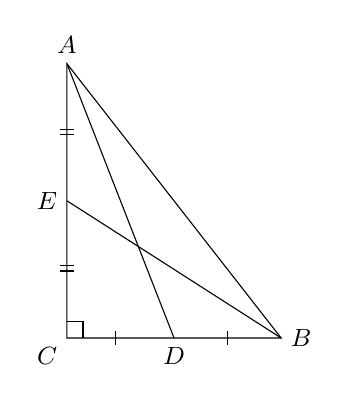
\begin{tikzpicture}[scale=0.17,font=\small]
\coordinate (C) at (0,0); \coordinate (B) at (16,0); \coordinate (A) at (0,20.49); \coordinate (D) at (8,0); \coordinate (E) at (0,10.25);
\draw (A)--(B)--(C)--cycle; \draw (A)--(D); \draw (B)--(E); \draw (0,1.2)--(1.2,1.2)--(1.2,0);
\draw (3.6,-0.5)--(3.6,0.5); \draw (12,-0.5)--(12,0.5); \draw (-0.5,5)--(0.5,5); \draw (-0.5,5.4)--(0.5,5.4); \draw (-0.5,15.2)--(0.5,15.2); \draw (-0.5,15.6)--(0.5,15.6);
\node[above] at (A) {$A$}; \node[right] at (B) {$B$}; \node[below left] at (C) {$C$}; \node[below] at (D) {$D$}; \node[left] at (E) {$E$};
\end{tikzpicture}}
\AB{$AB$ gipotenuza uzunligini toping.}{$ABC$ uçburçak yuzini toping.}}
\QQ{42}{Muntazam sakkizburçak tomoni $a=\sqrt{4-2\sqrt2}$.
\qfig{\begin{tikzpicture}[scale=1.2,font=\small]
\foreach \n/\a in {A/112.5,B/67.5,C/22.5,D/-22.5,E/-67.5,F/-112.5,G/-157.5,H/157.5} {\coordinate (\n) at (\a:1); \node at (\a:1.17) {$\n$};}
\fill[qfill] (A)--(D)--(E)--cycle;
\draw (A)--(B)--(C)--(D)--(E)--(F)--(G)--(H)--cycle; \draw (A)--(C); \draw (A)--(D); \draw (A)--(E);
\end{tikzpicture}}
\AB{$AC$ ning uzunligini toping.}{$S_{ADE}$ ni toping.}}
\QQ{43}{$ABCD$ parallelogrammda $DE$ balandlik va $E$ nuqta $AB$ ning örtasi, $F$ nuqta $DE$ ning örta nuqtasi, $G$ — $AC$ va $DE$ ning kesişiş nuqtasi. $ABCD$ parallelogrammning yuzi $48$ ga teng.
\qfig{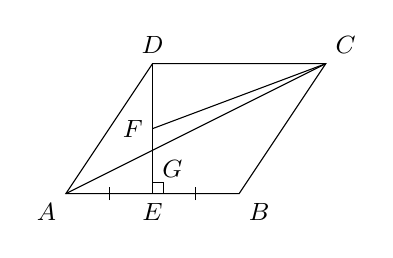
\begin{tikzpicture}[scale=0.55,font=\small]
\coordinate (A) at (0,0); \coordinate (E) at (2,0); \coordinate (B) at (4,0); \coordinate (D) at (2,3); \coordinate (C) at (6,3); \coordinate (F) at (2,1.5); \coordinate (G) at (2,1);
\draw (A)--(B)--(C)--(D)--cycle; \draw (D)--(E); \draw (A)--(C); \draw (F)--(C);
\draw (2,0.25)--(2.25,0.25)--(2.25,0); \draw (1,-0.15)--(1,0.15); \draw (3,-0.15)--(3,0.15);
\node[below left] at (A) {$A$}; \node[below] at (E) {$E$}; \node[below right] at (B) {$B$}; \node[above] at (D) {$D$}; \node[above right] at (C) {$C$}; \node[left] at (F) {$F$}; \node[below right] at (G) {$G$};
\end{tikzpicture}}
\AB{$CBEF$ törtburçak yuzasini toping.}{$CFG$ uçburçak yuzasining $AGE$ uçburçak yuzasiga nisbatini toping.}}
\QQ{44}{Yasovçisi katta asos tekisligi bilan $60^\circ$ burçak taşkil qiladigan va katta asos yuzasi $27\pi$ ga teng bölgan kesik konusga şar içki çizilgan.
\qfig{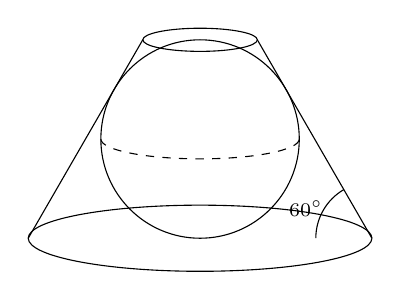
\begin{tikzpicture}[scale=0.42,font=\small]
\draw (0,0) ellipse (5.196 and 1); \draw (0,6) ellipse (1.732 and 0.35);
\draw (-5.196,0)--(-1.732,6); \draw (5.196,0)--(1.732,6); \draw (0,3) circle (3);
\draw[dashed] (-3,3) arc (180:360:3 and 0.6);
\node at (4.5,4.6) {}; \draw (3.5,0) arc (180:120:1.7); \node at (3.2,0.9) {\scriptsize$60^\circ$};
\end{tikzpicture}}
\AB{Kesik konus yon sirti yuzasini toping.}{Şar hajmini toping.}}
\QQ{45}{Usta parabola şaklidagi issiqxona qurdi va uni yaşindan himoya qiliş maqsadida $AB$ yaşin qaytargiç örnatdi. $CG=16$, $KL=6$, $BE=8$ va $AK$ — parabolaga urinma. $C$ — parabolaning eng baland nuqtasi, $KL\perp AB$ bölsa,
\qfig{\begin{tikzpicture}[xscale=0.3,yscale=0.13,font=\small]
\fill[qfill] plot[domain=0:8,samples=40] (\x,{16-(\x-4)^2})--cycle;
\draw (-7,0)--(12,0); \draw[thick,domain=0:8,samples=40] plot (\x,{16-(\x-4)^2});
\draw (0,0)--(0,36)--(9,0); \draw (0,36)--(-7,0); \draw (4,0)--(4,16); \draw (0,12)--(6,12);
\node[above] at (0,36) {$A$}; \node[below] at (0,0) {$B$}; \node[below] at (4,0) {$G$}; \node[below left=-1pt] at (8,0) {$E$}; \node[below right=-1pt] at (9,0) {$D$}; \node[below] at (-7,0) {$F$};
\node[above left] at (4,16) {$C$}; \node[left] at (0,12) {$L$}; \node[right] at (6,12.5) {$K$};
\end{tikzpicture}}
\AB{$\tg\angle ADE$ ni toping.}{$AB$ ning uzunligini toping.}}
\Javoblar{B C A D C B C B B C D A B B D A C D C C B A A A B B B C D A C A C A D}{%
\OK{36}{$7$}{$12$}\OK{37}{$\dfrac\pi{12}$}{$-\dfrac\pi6$}\OK{38}{$2$}{$0$}\OK{39}{$9$ ta}{$16$ ta}\OK{40}{$\dfrac45$}{$-\dfrac15$}%
\OK{41}{$26$}{$16\sqrt{105}$}\OK{42}{$2$}{$\sqrt2$}\OK{43}{$24$}{$1$}\OK{44}{$48\pi$}{$36\pi$}\OK{45}{$4$}{$36$}}
